\documentclass{article}
\usepackage[utf8]{inputenc}
\usepackage{graphicx}
\newcommand\tab[1][1cm]{\hspace*{#1}}

\title{TI}
\author{Sebastian Benkel}
\date{January 2017}

\begin{document}

1. Welche zwei Hauptaufgaben hat ein Betriebssystem?
\\
\\
Abstraktion von Ger\"ateeigenschaften(Alle Drucker lassen sich gleich verwenden, Standartinterfaces, etc.)

Unterst\"utzung des Mehrbenutzerbetriebs(Betriebsmittelverwaltung, Zuteilungsstrategien, etc)
\\
\\
2. Was ist ein Prozess?
\\
\\
Ein Programm in ausf\"uhrung(Kontrollfaden)
\\
\\
3. Wie ist ein Unix-Dateisystem strukturiert? Wie können Dateien darin (eindeutig) aufgefunden werden?
\\
\\
Es besteht aus Langlebigen Datenobjekten, die \"uber ihren eindeutigen Namen(Vollständige Dateinamen sind Pfadnamen vom Wurzelverzeichnis abwärts)(mehrere solcher Namen pro Datei m\"oglich) identifiziert werden k\"onnen. Die Struktur ist hierarchisch und Baumartig, l\"asst aber mehr als einen Pfad zur Datei zu.
\\
\\
4. Was ist ein symbolic link?
\\
\\
Ein Symbolic Link ist ein Pfadverweis auf eine Datei oder einen Ordner. Wird die Datei entfernt zeigt der Link an eine nicht existente Adresse.
\\      
\\
5. Ist das Unix-Dateisystem wirklich ein Baum? Begründung.
\\
\\
Nein, in einem Baum kann es keine zwei Wege auf die selbe Stelle geben. Im Unix-Dateisystem geht dies f\"ur Dateien(Hard Links)(Nicht f\"ur Ordner um Rekursion zu verhindern).
\\
\\
6. Welche Zugriffsrechte kann man auf eine Unix-Datei haben? Welche Dateiattribute steuern
dies, und wie?
\\
\\
Es gibt Read(lesen des Dateiinhalts. einsicht bei Ordnern), Write(ver\"andern des Dateiinhalts, Eintr\"age \"andern bei Ordnern), und Execute(ausf\"uhren der Datei als Programm, Zugriff auf Inhalt bei Ordnern) Rechte. diese werden in den Atributen der Datei vermerkt(f\"ur besitzer, Gruppe und Welt). \"Anderbar mit chmod
\\
\\
7. Welche Vorteile bietet es, auf Geräte in Unix wie auf Dateien zuzugreifen? Was versteht
man unter Ein-/Ausgabeumlenkung?
\\
\\
Textausgaben werden standartm\'a\ss ig in eine \"{}Standart-Ausgabedatei\"{} (das aktive Terminal(''stdout'')) geschrieben. diese kann durch andere Dateien ersetzt werden, so das Textausgabe direkt in Dateien umgelenkt werden k\"onnen.($>,>>.|$).
Dateiinhalt kann so an funktionen(sort, etc) \"ubergeben werden.
\\
\\
8. Welche Aufgabe hat ein Kommando-Interpreter (z.B. in Unix der Shell)?
\\
\\
Befehle entgegen zunehmen und umzusetzen, Prozesse abzubrechen, neue Prozesse aufzusetzen, generell Usereingaben umzusetzen.
\\
\\
9. Was machst Du, wenn Dir die genaue Semantik eines Unix-Kommandos entfallen ist?
\\
\\
\$ man Komandoname liefert die manpage
\\
\\
10. bla sei ein ausführbares Programm. Was ist der Unterschied zwischen dem Aufruf bla und
dem Aufruf bla \& in der Shell? Welche Auswirkungen hat dies, wenn bla von Standard
Input liest bzw. auf Standard Output schreibt? Gegeben sei der in Abbildung 1 dargestellte
Prozessbaum. Wie ändert er sich nach Eingeben der folgenden Kommandofolge im Shell?
init
bash
Abbildung 1: Prozessbaum
sleep 1000 \&
emacs \&
bash
date

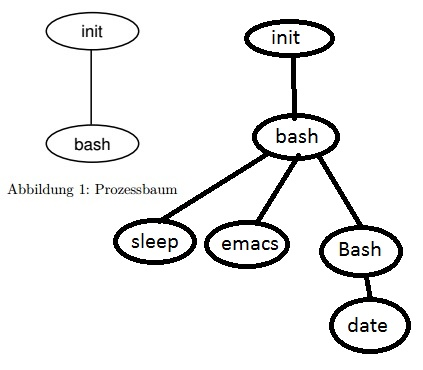
\includegraphics{Ti1.jpeg}
\\
\\
Der Aufruf bla \"ubergibt die Kontrolle der Komandozeile an den gestarteten Prozess, so das eingegebene Befehle nicht mehr ber\"ucksichtigt werden(bis auf Signale wie ctl-...). Der Aufruf & bla startet bla als Hintergrundprozess und die Kontrolle der Komandozeile wird nicht abgegeben. Eingaben werden weiter angenommen. Textausgaben von bla werden im Terminal ausgegeben(sehr un\"ubersichtlich). 
\\
\\
11. Nenne drei Beispiele für Informationen, die der Betriebssystemkern über einen Prozess
wissen muss.
\\
\\
Vaterprozess(PPID), Jobnummer(PID), Besitzer(UID),
\\
\\
12. Was ist eine Pipe?
\\
\\
Eine Pipe ist ein Buffer der die Ausgabe eines Prozesses mit der Eingabe eines Anderen Prozesses verbindet(stdin, stdout).
\\
\\
13. Wie macht man ein soeben editiertes Shell-File ausführbar?
\\
\\
chmod 1/chmod3/chmod5,chmod7...
\\
\\
14. In welche Bereiche (Segmente) ist der (virtuelle) Adressraum eines Programms in Ausführung in Unix unterteilt, und welche Eigenschaften kennzeichnen sie?
\\
\\
Text - hier liegt der code des Programms, sollte read-only sein.

Daten - hier liegen die (in Java, C++ durch  new) globalen vriablen des Programms, kann dynamisch erweitert werden(read + write)

Stack - hier wird der Status bei Prozeduraufrauf gerettet, die Parameter der Prozedur sowie Lokale Variablen der Prozedur (wächst/schrumpft dynamisch nach Bedarf) Es gibt einen Stackpointer um das Oberste Element anzuzeigen.(read + write)

Sie sind auf virtuelle Adressen abgebildet, d.h. werden im Arbeitsspeicher darauf gemapt.


Ungenutze Adressen - Hier liegt nichts, und es kann auch nicht zugrgriffen werden.
\\
\\
15. Wozu wird der Stack verwendet?
\\
\\
 hier wird der Status bei Prozeduraufrauf gerettet, die Parameter der Prozedur sowie Lokale Variablen der Prozedur (wächst/schrumpft dynamisch nach Bedarf) Es gibt einen Stackpointer um das Oberste Element anzuzeigen.
\\
\\
16. Welchem Zweck dienen Bibliotheken (Libraries)?
\\
\\
Libraries sind fertige Programmteile die einfach in ein Programm eingebettet werden um von ihnen genutzt zu werden(weniger schreibarbeit).
\\
\\
17. Welche Aufgabe erfüllt ein Linker?
\\
\\
Ein Linker erzeugt aus zusammengeh\"orenden .o Dateien eine Executable(Programm), mit gemeinsamem Adressraum und relativen call-adressen(call main() $\rightarrow$ call -116).
\\
\\
18. Wozu wird beim Assemblieren eine Symboltabelle angelegt?
\\
\\
Die Symboltabelle organisiert die Nutzung gemeinsamer Funktionen und Variablen. Wenn sie fertig gef\"ullt ist, beinhaltet sie einen Eintrag für jedes „sichtbare“ Symbol, bestehend aus:

\tab • Name des Symbols durch Verweis auf Startbyte in Stringtabelle

\tab • Typ (+Adresse)

Genutzt wird sie dann um Funktions- und Variablenaufrufe im Code durch relative Aufrufe zu ersetzen. Variablen werden an Adresse im Datensegment verlinkt. Um \"Uberladung bei Funktionen zu erm\"oglichen nutzt sie Namemangling(Parameterangaben am Namensende). Die eigentlichen Methodennamen liegen auf der Stringtabelle.  Wenn Das Programm fertig \"ubersetzt ist, kann die Symboltabelle, Stringtabelle und die Text/Data Relocation Tabelle gel\"oscht werden.
\\
\\
19. Welchen Vorteil hat es, Bibliotheken mit Position Independent Code zu versehen?
\\
\\
Der Code kann ausgef\"uhrt werden, auch wenn er nicht in der Originalzeile liegt. Library files werden von vielen Klassen parallel eingebunden und m\"ussen so nicht in jedem Programm in der selben zeile liegen.
\\
\\
20. Durch welche „Qualitätsmerkmale“ sollten Betriebssysteme gekennzeichnet sein? Nenne
Beispiele für konkurrierende Anforderungen.
\\
\\
Zuverlässigkeit:

\tab • Korrektheit - Verfügbarkeit

\tab • Sicherheit - Fehlertoleranz

\tab • Verfügbarkeit

\tab • Fehlertoleranz

\tab • Robustheit

Benutzerfreundlichkeit:

\tab • Verständlichkeit

\tab • Angemessenheit - Verständlichkeit

\tab • Vernünftiges Fehlerverhalten

Wartbarkeit und Flexibilität:

\tab • Testbarkeit

\tab • Erweiterbarkeit

\tab • Adaptierbarkeit

\tab • Portabilität

Leistungsfähigkeit:

\tab • Effektivität

\tab • Effizienz

Kosten - gegen alles
\\
\\
21. Worin unterscheidet sich der Kernel-Mode vom User-Mode (in Unix)? Warum wird diese
Unterscheidung getroffen?
\\
\\
Der Kermelmode hat seinen eigenen Adressraum(Text, Daten, Stack) den nur er betreten darf.

Eigenen Betriebssystem-Code den nur er ausf\"uhren darf. Dieser beinhaltet erweiterte funktionalit\"aten, eigene Maschineninstruktionen, er kann interupts unterdr\"ucken/aufschieben.

\\
\\
22. Was passiert in etwa bei einem Systemaufruf? (Reihenfolge der Arbeitsschritte.)
\\
\\
Das programm das den CPU benutzt wird pausiert und sein Zustand (User-Stack-Pointer (usp) auf den Kernel-Stack,
Register auf den Kernel-Stack (⇒ Kontext retten)) gerettet. Ggf. werden beim Interrupthandler interrupts Ausmaskiert(unterdr\"uckt), dann wird der Systemaufruf im Kernelmode abgearbeitet, es erfolgt ggf. Prozessumschaltung & Signalauslieferung, der Kernel-Stack wird aufgeräumt, es geht zur\"uck in den User-Mode, der User-Stack wird aufgeräumt und es geht zurück ins Anwendungsprogramm.
\\
\\
23. Was ist ein Interrupt? Nenne Beispiele für mögliche Interrupt-Quellen. Warum werden sie
unterschiedlich priorisiert? Wie wird ein Interrupt in etwa behandelt?
\\
\\
Ein Interrupt ist eine Aufforderung zur Systemunterbrechung um einen eiligen Auftrag auszuf\"ullen(keine Traps). Dazu geh\"poren clocktics, Tastatureingaben (begrenzter Buffer), Plattenauftr\"age, etc(in der Regel Prozessunabh\"angig). Sie werden prioritisiert, damit Zeitlritischere Interrupts weniger kritische Interrupts aussetzen k\"onnen(clocktick wichtiger als Plattenzugriff, da folgeinterrupts verpuffen). Interrupts laufen normalerweise wie folgt ab:

• i.d.R. nach Beendigung des aktuellen Befehlszyklus

• Retten des Prozesszustands

• nach Behandlung i.d.R. Rücksprung

\\
\\
24. Was ist ein Trap? Nenne Beispiele. Inwiefern unterscheiden sich Traps von Interrupts?
\\
\\
• aus prozessinternen Gründen(Plattenzugriff, read(), write())

• Division durch 0

• Zugriff auf eine illegale Adresse(ührt i.d.R. zum Programmabbruch)

• Zugriff auf Informationen, die z.Zt. nicht im Speicher stehen

W\"arend Interrupts meist nichts mit dem Programm in Ausf\"uhrung zu tun haben, sind Interrupts Systemaufrufe die freiwillig oder unfreiwillig vom laufenden Programm verursacht werden.
\\
\\
25. Was ist ein Signal? Nenne Beispiele für mögliche Signalquellen. Wie kann ein Prozess auf
ein Signal reagieren?
\\
\\
\\
\\
26. Beschreibe kurz einige Zustände, in denen sich ein (Unix-)Prozess befinden kann.
\\
\\
\\
\\
27. Nenne einige Randbedingungen, auf die man beim Entwurf eines Schedulers achten sollte.
Wie sollten rechenintensive bzw. Ein-/Ausgabe-intensive Prozesse dabei behandelt werden?
\\
\\
\\
\\
28. Wie könnte man mit Hilfe eines Round-Robin-Schedulers Prozessprioritäten „simulieren“?
\\
\\
\\
\\
29. Warum bestehen die Sleep-Queue und die Run-Queue in Unix nicht aus jeweils einer
einzigen Warteschlange? Wie sind sie stattdessen organisiert?
\\
\\
\\
\\
30. Warum werden die Zustandsinformationen eines Unix-Prozesses teilweise in der ProcStruktur und teilweise in der User-Struktur abgelegt? Nenne jeweils drei charakteristische
Beispiele für Angaben darin.
\\
\\
\\
\\
31. Skizziere kurz die Prozesserzeugung in Unix. Welche Rolle spielen die Systemaufrufe fork()
und exec()?
\\
\\
\\
\\
32. Wie erfährt ein Unix-Prozess, ob ein Kindprozess terminiert ist? Wozu gibt es in Unix den
Prozesszustand SZOMB („Zombie“)?
\\
\\
\\
\\
33. Welche Vor- und Nachteile hat der First-Fit- bzw. der Best-Fit-Algorithmus zur Speicherverwaltung? Wie arbeitet der Buddy-Algorithmus in etwa?
\\
\\
\\
\\
34. Wozu bieten Systeme eine Speicherhierarchie an? Welche Beobachtung über den Speicherzugriff realer Programme liegt dem zugrunde? Welche verschiedenen Arten von Speiche
werden typischerweise bereitgestellt?
\\
\\
\\
\\
35. Warum ist es in der Regel nicht sinnvoll, den Adressraum eines Prozesses in einem Stück
im Hauptspeicher abzulegen?
\\
\\
\\
\\
36. Was versteht man unter Paging, was unter Segmentierung? Wo tritt interne Fragmentierung,
wo externe Fragmentierung auf? Was ist das?
\\
\\
\\
\\
37. Aus welchen Teilen besteht eine virtuelle Adresse zumeist? Wie ermittelt sich daraus die
entsprechende Hauptspeicheradresse, d. h. wie läuft die Adressverwaltung in etwa ab?
\\
\\
\\
\\
38. Wie können mehrere Prozesse mit Hilfe virtueller Adressierung auf dieselben Programmstücke (oder auch Datenbereiche) zugreifen?
\\
\\
\\
\\
39. Warum ist ein perfekter Algorithmus zur Verdrängung von Pages aus dem Hauptspeicher
nicht realisierbar? Wie arbeiten die folgenden Algorithmen in etwa:
a) FIFO (First-In-First-Out),
b) LFU (Least-Frequently-Used),
c) LRU (Least-Recently-Used)?
\\
\\
\\
\\
40. In welche dieser Kategorien kann man NRU (Not-Recently-Used) einordnen? Wie arbeitet
der Clock-Hand-Algorithmus?
\\
\\
\\
\\
41. Was passiert, wenn die Umlaufzeit des Zeigers beim Clock-Hand-Algorithmus zu groß bzw.
zu klein gewählt wird? Wie kann ein zweiter Zeiger den Algorithmus verbessern?
\\
\\
\\
\\
42. Was ist Swapping? Warum wenden auch Paging-Systeme dieses Verfahren an bzw. unter
welcher Bedingung?
\\
\\
\\
\\
43. Wie kann man die Vorteile von Paging und Segmentierung kombinieren?
\\
\\
\\
\\
44. Wozu bzw. wo wird bei der Speicherverwaltung häufig ein Assoziativspeicher eingesetzt?
\\
\\
\\
\\
45. Beschreibe kurz die Zugriffsoperationen open(), close(), lseek(), read() und write()
auf ein Unix-Filesystem. Welche Rolle spielt dabei der Filedeskriptor?
\\
\\
\\
\\
46. Wie sieht die Struktur des Unix-V7-Dateisystems auf der Platte in etwa aus? Warum erfolgt
die Verwaltung der Freispeicherliste über Indirekt-Blöcke?
\\
\\
\\
\\
47. Welche Angaben enthält ein Inode? Welche Angaben enthält eine Verzeichnis-Datei (Euch
besser bekannt als „Directory“)?
\\
\\
\\
\\
48. Welche Aufgaben hat der Buffer Cache in Unix?
\\
\\
\\
\\
49. Was geschieht durch den Systemaufruf mount() in etwa?
\\
\\
\\
\\
50. Welche Vorteile bietet es, Dateien mit dem Unix-Systemaufruf mmap() in den virtuellen
Adressraum eines Prozesses abzubilden?
\\
\\
\\
\\
51. Wie ist eine Platte intern organisiert? Wie wirkt sich dies auf den Informationszugriff aus?
Wie geht das Unix Fast File System damit um?
\\
\\
\\
\\
52. Welche Vorteile bietet eine vereinheitlichte Betriebssystemschnittstelle zum Zugriff auf
Geräte? Wie sieht sie in Unix in etwa aus?
\\
\\
\\
\\
53. Was ist ein Gerätetreiber, was ein Geräte-Controller? Welche Aufgaben haben sie?
\\
\\
\\
\\
54. Warum erfolgt der Zugriff auf Geräte häufig über Warteschlangen? Wozu besitzen diese in
der Regel eine High Water Mark bzw. eine Low Water Mark?
\\
\\
\\
\\
55. Worin unterscheidet sich DMA (Direct Memory Access) von Programmed I/O?
\\
\\
\\
\\
56. Warum werden Terminal-Treiber in Unix parametrisiert? Nenne typische Parameter.
\\
\\
\\
\\
57. Skizziere kurz einige Probleme des nebenläufigen Zugriffs auf Betriebsmittel.
\\
\\
\\
\\
58. Grenze die Begriffe Nebenläufigkeit, Quasi-Parallelität und Parallelität voneinander ab.
Was verstehen wir unter Nichtdeterminismus?
\\
\\
\\
\\
59. Welche Nebenläufigkeitseigenschaften bzw. -probleme werden durch die drei folgenden
„klassischen“ Szenarien ausgedrückt:
• Erzeuger/Verbraucher (Producer/Consumer),
• Leser/Schreiber (Reader/Writer),
• Speisende Philosophen (Dining Philosophers)?
\\
\\
\\
\\
60. Was ist ein Thread? Skizziere ein sinnvolles Anwendungsbeispiel für die Verwendung
mehrerer Threads innerhalb eines Prozesses.
\\
\\
\\
\\
61. Grenze den Thread-Begriff gegen den UNIX-Prozess-Begriff ab (Adressraum, Zustandsinformationen usw.). Was haben Light-Weight-Prozesse (LWPs) damit zu tun?
\\
\\
\\
\\
62. Die Routinen pthread_create(), pthread_join(), pthread_exit() realisieren die Erzeugung und Termination von Threads in der UNIX-Multithreading-Umgebung. Vergleiche
ihre Funktionalität mit den Systemaufrufen zur Erzeugung und Termination von Prozessen
(wait(), fork() und exit()). Warum arbeitet pthread_create() deutlich anders als
fork()?
\\
\\
\\
\\
63. Was versteht man unter einseitiger Synchronisation bzw. mehrseitiger Synchronisation?
Gib jeweils ein Anwendungsbeispiel an.
\\
\\
\\
\\
64. Was ist ein kritischer Abschnitt? Wie kann man den gegenseitigen Ausschluss gewährleisten?
Warum ist ein Unterbrechungsausschluss dabei nicht immer das geeignete Mittel?
\\
\\
\\
\\
65. Nach welchen Kriterien wird die Korrektheit bzw. Güte von Locking-Algorithmen bewertet?
Wie geht man dabei vor?
\\
\\
\\
\\
66. Warum sollte man die Bewertung von Locking-Algorithmen auf der Grundlage von unteilbaren Operationen durchführen?
\\
\\
\\
\\
67. Auf welche verschiedene Arten kann man Verklemmungen angehen? Wie arbeitet der
Bankiersalgorithmus?
\\
\\
\\
\\
68. Wie kann man eine einseitige Synchronisation mit Hilfe von wait() und signal() vornehmen? Wie kann man diese Primitiven in etwa auf lock() und unlock() abbilden?
\\
\\
\\
\\
69. Grenze die Begriffe aktives und blockierendes Warten gegeneinander ab.
\\
\\
\\
\\
70. In einer UNIX-Multiprozessorumgebung können mehrere Prozesse nebenläufig sleep()
aufrufen. Warum ist dies ein kritischer Abschnitt? Warum kann man ihn nicht einfach
dadurch schützen, dass man den Aufruf von sleep() von einem Spinlock umgibt? Was
wird man stattdessen tun?
\\
\\
\\
\\
71. Welche zusätzlichen Eigenschaften zeichnen Semaphore gegenüber blockierenden Locks
aus?
\\
\\
\\
\\
72. Wie wird eine einseitige bzw. eine mehrseitige Synchronisation durch Semaphore ausgedrückt?
\\
\\
\\
\\
73. Wie können Semaphore zur Lösung des Problems der speisenden Philosophen eingesetzt
werden? In welches Problem wird eine allzu einfache „Implementierung“ laufen?
\\
\\
\\
\\
74. Warum bietet eine einfache Semaphor-Implementierung mit den UNIX-eigenen sleep-
/wakeup-Routinen keine vollständige Semaphor-Semantik? Welche zusätzlichen Maßnahmen
müsste man ergreifen?
\\
\\
\\
\\
75. Welche Probleme gibt es mit „fairen Semaphoren“? Was sind „Konvois“, und was sind
„donnernde Herden“?
\\
\\
\\
\\
76. Was ist ein Monitor? Unter welchen Bedingungen wird ein Monitor betreten bzw. wieder
verlassen?
\\
\\
\\
\\
77. Aus welchen Komponenten besteht ein Petrinetz (mit Marken)? Was kann man damit
beschreiben?
\\
\\
\\
\\
78. Wie kann man durch ein Petrinetz typische Synchronisationsvorschriften ausdrücken:
a) Sequenz,
b) Beschränkte Nebenläufigkeit,
c) Unabhängigkeit?
\\
\\
\\
\\
79. Was kennzeichnet lebendige bzw. todesgefährdete Petrinetze?
\\
\\
\\
\\
80. Was versteht man unter synchronem bzw. asynchronem Nachrichtenaustausch? Inwiefern
sind diese beiden Kommunikationsformen aufeinander abbildbar?
\\
\\
\\
\\
81. Wie kann man die Synchronisationseigenschaften von synchronem bzw. asynchronem
Nachrichtenaustausch mit Semaphoren modellieren?
\\
\\
\\
\\
82. Wozu verwendet man Kanäle bzw. Ports? Was ist das?
\\
\\
\\
\\
83. Was ist ein guarded command? Warum kann die Verwendung eines solchen Konzepts gerade
in Zusammenhang mit Nachrichtenaustauschvorgängen interessant sein?
\\
\\
\\
\\
84. Wie arbeitet der Korridor-Algorithmus zum Überwachen mehrerer Eingabequellen in etwa?
\\
\\
\\
\\
85. Worin unterscheiden sich die Eigenschaften der folgenden UNIX-Mechanismen zur Interprozesskommunikation:
• Pipes,
• Named Pipes,
• Sockets?
\\
\\
\\
\\
86. Wie lassen sich die Kommunikationseigenschaften von Sockets mit normaler Briefpost und
Telefongesprächen vergleichen?
\\
\\
\\
\\
87. Wie lässt sich der Zugriff auf Sockets in die generische Systemaufrufschnittstelle zum Zugriff
auf Dateien einordnen?
\\
\\
\\
\\
88. Warum kommt dem Adressierungsproblem in der Interprozesskommunikation eine so große
Bedeutung zu? In welche zwei Teile zerfällt eine Adressangabe typischerweise?
\\
\\
\\
\\
89. Was ist ein (Kommunikations-)Protokoll?
\\
\\
\\
\\
90. Skizziere kurz einige typische Kommunikationsprobleme und je einen Lösungsvorschlag im
Rahmen eines entsprechenden Protokolls.
\\
\\
\\
\\
91. Skizziere einige Eigenschaften typischer Netztopologien.
\\
\\
\\
\\
92. Welche besondere Bedeutung kommt dem Protokoll IP zu?
\\
\\
\\
\\
93. Was ist ein Remote Procedure Call (RPC), und welche Parameter wird man typischerweise
dabei übergeben? Was haben RPCs mit dem Client/Server-Modell zu tun?
\\
\\
\\
\\
94. Nenne einige absichtliche und unabsichtliche Angriffe auf Hardware, Software und/oder
Daten. Wie können solche Angriffe klassifiziert werden?
\\
\\
\\
\\
95. Welche grundsätzlichen Sicherheitsziele kann man unterscheiden? Was ist eine Sicherheitspolitik?
\\
\\
\\
\\
96. Auf welche verschiedenen Arten kann sich ein Benutzer authentifizieren?
\\
\\
\\
\\
98. Welche Komponenten enthält eine Zugriffskontrollmatrix? Wie ordnen sich die Dateizugriffsrechte in UNIX in dieses Schema ein?
\\
\\
\\
\\
99. Charakterisiere symmetrische und asymmetrische Verschlüsselungsverfahren. Wie können sie
zur Realisierung einer Vertraulichkeit eingesetzt werden? Warum werden häufig Mischformen
eingesetzt?

\end{document}
